\documentclass[preprint, 3p,
authoryear]{elsarticle} %review=doublespace preprint=single 5p=2 column
%%% Begin My package additions %%%%%%%%%%%%%%%%%%%

\usepackage[hyphens]{url}

  \journal{Software X} % Sets Journal name

\usepackage{lineno} % add

\usepackage{graphicx}
%%%%%%%%%%%%%%%% end my additions to header

\usepackage[T1]{fontenc}
\usepackage{lmodern}
\usepackage{amssymb,amsmath}
\usepackage{ifxetex,ifluatex}
\usepackage{fixltx2e} % provides \textsubscript
% use upquote if available, for straight quotes in verbatim environments
\IfFileExists{upquote.sty}{\usepackage{upquote}}{}
\ifnum 0\ifxetex 1\fi\ifluatex 1\fi=0 % if pdftex
  \usepackage[utf8]{inputenc}
\else % if luatex or xelatex
  \usepackage{fontspec}
  \ifxetex
    \usepackage{xltxtra,xunicode}
  \fi
  \defaultfontfeatures{Mapping=tex-text,Scale=MatchLowercase}
  \newcommand{\euro}{€}
\fi
% use microtype if available
\IfFileExists{microtype.sty}{\usepackage{microtype}}{}
\usepackage[]{natbib}
\bibliographystyle{plainnat}

\ifxetex
  \usepackage[setpagesize=false, % page size defined by xetex
              unicode=false, % unicode breaks when used with xetex
              xetex]{hyperref}
\else
  \usepackage[unicode=true]{hyperref}
\fi
\hypersetup{breaklinks=true,
            bookmarks=true,
            pdfauthor={},
            pdftitle={An R-based end-to-end optimization program for multi-product multi-period multi-supplier raw-material selection and composition, and order quantity problem with minimum one-year order quantity contract},
            colorlinks=false,
            urlcolor=blue,
            linkcolor=magenta,
            pdfborder={0 0 0}}

\setcounter{secnumdepth}{5}
% Pandoc toggle for numbering sections (defaults to be off)

% Pandoc syntax highlighting
\usepackage{color}
\usepackage{fancyvrb}
\newcommand{\VerbBar}{|}
\newcommand{\VERB}{\Verb[commandchars=\\\{\}]}
\DefineVerbatimEnvironment{Highlighting}{Verbatim}{commandchars=\\\{\}}
% Add ',fontsize=\small' for more characters per line
\usepackage{framed}
\definecolor{shadecolor}{RGB}{248,248,248}
\newenvironment{Shaded}{\begin{snugshade}}{\end{snugshade}}
\newcommand{\AlertTok}[1]{\textcolor[rgb]{0.94,0.16,0.16}{#1}}
\newcommand{\AnnotationTok}[1]{\textcolor[rgb]{0.56,0.35,0.01}{\textbf{\textit{#1}}}}
\newcommand{\AttributeTok}[1]{\textcolor[rgb]{0.77,0.63,0.00}{#1}}
\newcommand{\BaseNTok}[1]{\textcolor[rgb]{0.00,0.00,0.81}{#1}}
\newcommand{\BuiltInTok}[1]{#1}
\newcommand{\CharTok}[1]{\textcolor[rgb]{0.31,0.60,0.02}{#1}}
\newcommand{\CommentTok}[1]{\textcolor[rgb]{0.56,0.35,0.01}{\textit{#1}}}
\newcommand{\CommentVarTok}[1]{\textcolor[rgb]{0.56,0.35,0.01}{\textbf{\textit{#1}}}}
\newcommand{\ConstantTok}[1]{\textcolor[rgb]{0.00,0.00,0.00}{#1}}
\newcommand{\ControlFlowTok}[1]{\textcolor[rgb]{0.13,0.29,0.53}{\textbf{#1}}}
\newcommand{\DataTypeTok}[1]{\textcolor[rgb]{0.13,0.29,0.53}{#1}}
\newcommand{\DecValTok}[1]{\textcolor[rgb]{0.00,0.00,0.81}{#1}}
\newcommand{\DocumentationTok}[1]{\textcolor[rgb]{0.56,0.35,0.01}{\textbf{\textit{#1}}}}
\newcommand{\ErrorTok}[1]{\textcolor[rgb]{0.64,0.00,0.00}{\textbf{#1}}}
\newcommand{\ExtensionTok}[1]{#1}
\newcommand{\FloatTok}[1]{\textcolor[rgb]{0.00,0.00,0.81}{#1}}
\newcommand{\FunctionTok}[1]{\textcolor[rgb]{0.00,0.00,0.00}{#1}}
\newcommand{\ImportTok}[1]{#1}
\newcommand{\InformationTok}[1]{\textcolor[rgb]{0.56,0.35,0.01}{\textbf{\textit{#1}}}}
\newcommand{\KeywordTok}[1]{\textcolor[rgb]{0.13,0.29,0.53}{\textbf{#1}}}
\newcommand{\NormalTok}[1]{#1}
\newcommand{\OperatorTok}[1]{\textcolor[rgb]{0.81,0.36,0.00}{\textbf{#1}}}
\newcommand{\OtherTok}[1]{\textcolor[rgb]{0.56,0.35,0.01}{#1}}
\newcommand{\PreprocessorTok}[1]{\textcolor[rgb]{0.56,0.35,0.01}{\textit{#1}}}
\newcommand{\RegionMarkerTok}[1]{#1}
\newcommand{\SpecialCharTok}[1]{\textcolor[rgb]{0.00,0.00,0.00}{#1}}
\newcommand{\SpecialStringTok}[1]{\textcolor[rgb]{0.31,0.60,0.02}{#1}}
\newcommand{\StringTok}[1]{\textcolor[rgb]{0.31,0.60,0.02}{#1}}
\newcommand{\VariableTok}[1]{\textcolor[rgb]{0.00,0.00,0.00}{#1}}
\newcommand{\VerbatimStringTok}[1]{\textcolor[rgb]{0.31,0.60,0.02}{#1}}
\newcommand{\WarningTok}[1]{\textcolor[rgb]{0.56,0.35,0.01}{\textbf{\textit{#1}}}}

% tightlist command for lists without linebreak
\providecommand{\tightlist}{%
  \setlength{\itemsep}{0pt}\setlength{\parskip}{0pt}}

% From pandoc table feature
\usepackage{longtable,booktabs,array}
\usepackage{calc} % for calculating minipage widths
% Correct order of tables after \paragraph or \subparagraph
\usepackage{etoolbox}
\makeatletter
\patchcmd\longtable{\par}{\if@noskipsec\mbox{}\fi\par}{}{}
\makeatother
% Allow footnotes in longtable head/foot
\IfFileExists{footnotehyper.sty}{\usepackage{footnotehyper}}{\usepackage{footnote}}
\makesavenoteenv{longtable}





\begin{document}


\begin{frontmatter}

  \title{An R-based end-to-end optimization program for multi-product
multi-period multi-supplier raw-material selection and composition, and
order quantity problem with minimum one-year order quantity contract}
    \author[lala]{Mohammad Rizka Fadhli%
  \corref{cor1}%
  }
   \ead{20921004@mahasiswa.itb.ac.id} 
    \author[lili]{Saladin Uttunggadewa%
  %
  }
  
    \author[lulu]{Rieske Hadianti%
  %
  }
  
    \author[lili]{Sri Redjeki Pudjaprasetya%
  %
  }
  
      \affiliation[lala]{Magister of Computational Sciences Program,
Faculty of Mathematics and Natural Sciences, Institut Teknologi Bandung}
    \affiliation[lili]{Faculty of Mathematics and Natural Sciences,
Institut Teknologi Bandung}
    \affiliation[lulu]{Center for Mathematical Modeling and Simulation,
Institut Teknologi Bandung}
    \cortext[cor1]{Corresponding author}
  
  \begin{abstract}
  This paper concerns the optimization model for a multi product multi
  period raw-material selection and composition, and order quantity
  problem faced by a beverage company. There are some criteria in raw
  material selection, which we accommodate all the criteria in the
  objective function. There are a number of suppliers, and one of the
  decision criteria is minimum one-year order quantity contracts between
  the company and the suppliers. The actual one-year demand of raw
  materials may deviate significantly from the minimum one-year order
  quantities. In this paper, we derive a function that can be regarded
  as a penalty function in order to maintain the total order quantities
  in one year fulfill the minimum one-year order quantity contracts.
  This penalty function is a part of the objective function, and can be
  relaxed once the the minimum one-year order quantity contracts are
  fulfilled. This optimization problem defined as mixed integer linear
  programming. We create an R-based end-to-end program to solve this
  optimization problem. Using various data inputs such as raw-material
  details, product's raw-material composition, and products demand, the
  end results of the program is weekly raw-material order allocation and
  composition. This program can be used in various manufacture industry.
  \end{abstract}
    \begin{keyword}
    inventory control \sep multi criteria raw-material
selection \sep mix-integer linear programming \sep 
    R programming
  \end{keyword}
  
 \end{frontmatter}

\hypertarget{introduction}{%
\section{Introduction}\label{introduction}}

This paper concerns the optimization model for supplier selection, order
allocation, and raw-material composition in a beverage company that
produces a large number of drink powders. There are a number of
suppliers that can provide the same key raw material of the drink
powders, but the color or some physical characteristics are slightly
different so we may assume those raw materials are different. The drink
powders produced by this company, which in the remainder of this paper
are called items, can be classified into two classes of items.

\begin{itemize}
\tightlist
\item
  The first class consists of items that can be produced by using
  exactly a single type of raw material.
\item
  The second class consists of more flexible items, where each item in
  this class can be produced by using one raw material or by using a
  composition of a number of raw materials. For each item in this class,
  we then have a set of possible raw materials. The sets of possible
  materials may vary from one to the other.
\end{itemize}

In order to avoid supply disruption, the company decides to use multiple
sources for these raw materials. The company has established selection
criteria for each raw material, which are based on the estimated
one-year total demand of raw materials and a subjective assessment of
whether the raw material cannot be substituted, price, service, and the
minimum order required for each purchase. After determining the score
for each raw material, the company decided to make contracts or
agreements with six suppliers. Each contract stated the unit price price
and the minimum order quantity within a year. Based on these contracts,
production planning and inventory control of raw materials are carried
out.

The estimated total one-year demand for items is obtained from the
forecasting process performed yearly. This forecasting process yields
the monthly total demand for items, which is time varying. But at the
production level, the company refines the monthly total demand on a
monthly basis as a response to some disruptions such as sudden
additional requests due to flash sales practices in e-commerce, and
others.

Once the demand for items for a month is issued, the company must
perform the decision for purchasing the raw materials from some
suppliers. This purchase decision from a supplier includes purchase for
four serial deliveries one week apart. The first delivery must be no
later than 17 days before the following month's start. The period of 17
days here is the total time required for the company's internal
inspection and preparation of raw materials.

This decision process is a complex one since there are a large number of
items that have to be produced which mostly belong to the second class,
and the monthly demand may vary. Additionally, the company imposes a
production regulation for the second class of items as a result of the
multiple-sources policy, which states that each item in the second class
must be produced using a composition of at least two types of the
corresponding possible raw materials. The decision process must be
performed carefully in order to obtain results in the form of:

\begin{itemize}
\tightlist
\item
  which raw materials are purchased along with the delivery size for
  every four corresponding weeks,
\item
  the composition of raw materials for every item in the second class
  which has to be produced,
\end{itemize}

while minimizing the total inventory cost.

The company developed a decision support system for this monthly
decision process, which is developed based on an optimization model.

\newpage

\hypertarget{hapus}{%
\section{Hapus}\label{hapus}}

Please make sure that your manuscript follows the guidelines in the
Guide for Authors of the relevant journal. It is not necessary to
typeset your manuscript in exactly the same way as an article, unless
you are submitting to a camera-ready copy (CRC) journal.

For detailed instructions regarding the elsevier article class, see
\url{https://www.elsevier.com/authors/policies-and-guidelines/latex-instructions}

\hypertarget{bibliography-styles}{%
\section{Bibliography styles}\label{bibliography-styles}}

Here are two sample references: \citet{Feynman1963118}.

uji coba \citep{Dirac1953888}

By default, natbib will be used with the \texttt{authoryear} style, set
in \texttt{classoption} variable in YAML. You can sets extra options
with \texttt{natbiboptions} variable in YAML header. Example

\begin{Shaded}
\begin{Highlighting}[]
\FunctionTok{natbiboptions}\KeywordTok{:}\AttributeTok{ longnamesfirst,angle,semicolon}
\end{Highlighting}
\end{Shaded}

There are various more specific bibliography styles available at
\url{https://support.stmdocs.in/wiki/index.php?title=Model-wise_bibliographic_style_files}.
To use one of these, add it in the header using, for example,
\texttt{biblio-style:\ model1-num-names}.

\hypertarget{using-csl}{%
\subsection{Using CSL}\label{using-csl}}

If \texttt{citation\_package} is set to \texttt{default} in
\texttt{elsevier\_article()}, then pandoc is used for citations instead
of \texttt{natbib}. In this case, the \texttt{csl} option is used to
format the references. Alternative \texttt{csl} files are available from
\url{https://www.zotero.org/styles?q=elsevier}. These can be downloaded
and stored locally, or the url can be used as in the example header.

\hypertarget{equations}{%
\section{Equations}\label{equations}}

Here is an equation: \[ 
  f_{X}(x) = \left(\frac{\alpha}{\beta}\right)
  \left(\frac{x}{\beta}\right)^{\alpha-1}
  e^{-\left(\frac{x}{\beta}\right)^{\alpha}}; 
  \alpha,\beta,x > 0 .
\]

Here is another: \begin{align}
  a^2+b^2=c^2.
\end{align}

Inline equations: \(\sum_{i = 2}^\infty\{\alpha_i^\beta\}\)

\hypertarget{figures-and-tables}{%
\section{Figures and tables}\label{figures-and-tables}}

Figure \ref{fig2} is generated using an R chunk.

\begin{figure}

{\centering 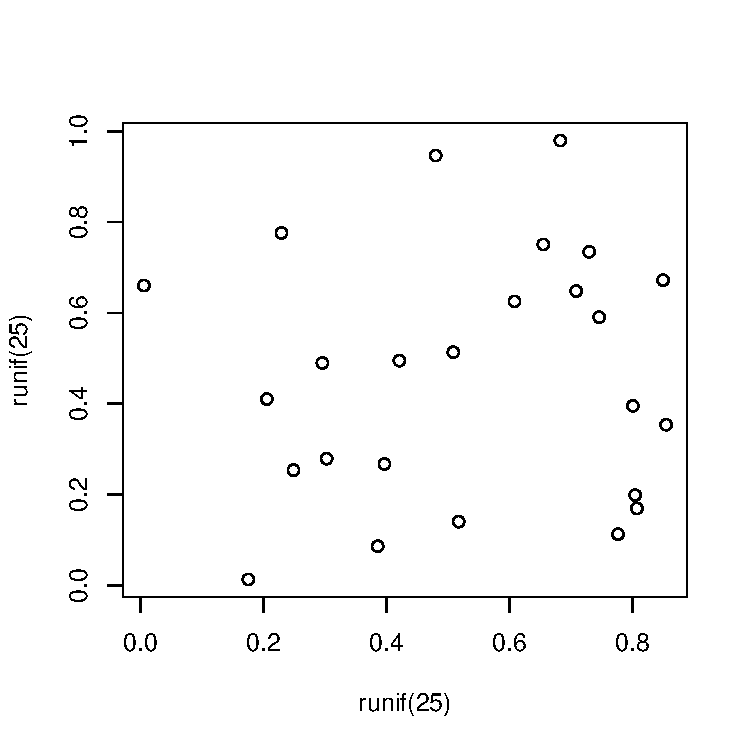
\includegraphics[width=0.5\linewidth]{Manuscript_files/figure-latex/fig2-1} 

}

\caption{\label{fig2}A meaningless scatterplot.}\label{fig:fig2}
\end{figure}

\hypertarget{tables-coming-from-r}{%
\section{Tables coming from R}\label{tables-coming-from-r}}

Tables can also be generated using R chunks, as shown in Table
\ref{tab1} for example.

\begin{Shaded}
\begin{Highlighting}[]
\NormalTok{knitr}\SpecialCharTok{::}\FunctionTok{kable}\NormalTok{(}\FunctionTok{head}\NormalTok{(mtcars)[,}\DecValTok{1}\SpecialCharTok{:}\DecValTok{4}\NormalTok{], }
    \AttributeTok{caption =} \StringTok{"}\SpecialCharTok{\textbackslash{}\textbackslash{}}\StringTok{label\{tab1\}Caption centered above table"}
\NormalTok{)}
\end{Highlighting}
\end{Shaded}

\begin{longtable}[]{@{}lrrrr@{}}
\caption{\label{tab1}Caption centered above table}\tabularnewline
\toprule()
& mpg & cyl & disp & hp \\
\midrule()
\endfirsthead
\toprule()
& mpg & cyl & disp & hp \\
\midrule()
\endhead
Mazda RX4 & 21.0 & 6 & 160 & 110 \\
Mazda RX4 Wag & 21.0 & 6 & 160 & 110 \\
Datsun 710 & 22.8 & 4 & 108 & 93 \\
Hornet 4 Drive & 21.4 & 6 & 258 & 110 \\
Hornet Sportabout & 18.7 & 8 & 360 & 175 \\
Valiant & 18.1 & 6 & 225 & 105 \\
\bottomrule()
\end{longtable}

\renewcommand\refname{References}
\bibliography{mybibfile.bib}


\end{document}
